\section{The Sen limit of F-theory}\label{sec:senlimit}

Sen \cite{Sen96ftheory} showed that F-theory on an elliptic K3 surface, at the point of its moduli space where the Weierstrass model $y^2 = x^3 + f(z)x + g(z)$ has constant modulus $\tau$ and four $D_4$ singular fibres, is the type IIB orientifold on $T^2/\ZZ_2$ with four orientifold seven-planes and four D7-branes on each, with gauge group $SO(8)^4$ and constant coupling; and that moving away from this point, in a one-parameter family $f = -3h^2 + \eps\eta$, $g = -2h^3 + \eps h\eta - \tfrac{1}{12}\eps^2\chi$ with $\eps\to0$, the coupling becomes weak away from the loci $h=0$, which are the orientifold planes, while the discriminant $\Delta = -9\eps^2 h^2(\eta^2 - h\chi) + O(\eps^3)$ places the D7-branes on $\eta^2 = h\chi$. In \cite{Sen97orientifold} the same expansion was applied to F-theory on elliptic Calabi--Yau threefolds and fourfolds over a base $B$, with $h,\eta,\chi$ sections of $K_B^{-2}, K_B^{-4}, K_B^{-6}$: the statement is that F-theory on such a Calabi--Yau has a weak coupling limit which is type IIB on the double cover of $B$ branched along $h=0$, with the orientifold projection, O7-planes on $h=0$ and D7-branes on $\eta^2=h\chi$.

\begin{theorem}[scope of the weak-coupling expansion]\label{thm:senlimitk3}
For $f=-3h^2+\eps\eta$ and $g=-2h^3+\eps h\eta-\eps^2\chi/12$, one has
\begin{align}
4f^3+27g^2={}&-9\eps^2h^2(\eta^2-h\chi)\nonumber\\
&+\eps^3(4\eta^3-\tfrac92h\eta\chi)+\tfrac3{16}\eps^4\chi^2.
\end{align}
At points with $h(\eta^2-h\chi)\ne0$, the modular invariant $j\propto f^3/(4f^3+27g^2)$ diverges as $\eps^{-2}$. This is a generic-point limit, not a smooth elliptic fibration at $\eps=0$: its discriminant vanishes identically there. The perturbative orientifold and D7 interpretation is the construction in \cite{Sen96ftheory,Sen97orientifold}. The generic O7 monodromy is $-T^{-4}$ in the convention of \cite{Sen97orientifold}; the enhanced O7 with four coincident D7-branes has combined monodromy $-I$.
\end{theorem}
\begin{proof}
The discriminant identity follows by expansion; the leading nonzero coefficient gives the asserted growth. The two monodromies concern different configurations: adding the four D7 monodromies $T^4$ cancels the $T^{-4}$ factor. A Kodaira type cannot be read from the everywhere-degenerate central fibre as though it were an ordinary smooth family.
\end{proof}

\begin{verdict}[claim 22]
Established in the stated geometric and physical framework. The constant-coupling $SO(8)^4$ model and the generic weak-coupling family are related constructions, not identical fibre configurations.
\end{verdict}

\begin{proposition}[base divisor and double-cover divisor]\label{prop:senlimitcy}
Suppose $h,\eta$ are local coordinates near $h=\eta=0$ on a smooth base and $\chi$ is nonzero there. The divisor $D_B=\{\eta^2-h\chi=0\}$ on the base is smooth at that point. On the smooth orientifold double cover $X=\{\xi^2=h\}$ its pullback is
\[
D_X=\{\eta^2-\xi^2\chi=0\},
\]
which is singular along $\xi=\eta=0$. Where $\chi$ is a unit it has two local branches. At a transverse triple locus $\xi=\eta=\chi=0$ in a three-dimensional cover, its local equation is the Whitney pinch form $u^2=v^2w$.
\end{proposition}
\begin{proof}
For $F=\eta^2-h\chi$, at $h=\eta=0$ one has $dF=-\chi\,dh\ne0$. On the cover, the three derivatives of $G=\eta^2-\xi^2\chi$ in these coordinates are $2\eta,-2\xi\chi,-\xi^2$, all zero on the stated double locus. A unit $\chi$ has a local analytic square root, so $G=(\eta-\xi\sqrt\chi)(\eta+\xi\sqrt\chi)$. The transverse triple locus gives the pinch form. This is the distinction used in the D7 analysis of \cite{CDE09}.
\end{proof}

\begin{proposition}[a non-Higgsable divisor is not a sufficient obstruction]\label{prop:i0star}
In a local chart let $s=0$ be a divisor and take
\[
h=s h_1,\qquad\eta=s^2\eta_2,\qquad\chi=s^3\chi_3.
\]
Then $f=s^2F_\eps$, $g=s^3G_\eps$, with
\[
F_\eps=-3h_1^2+\eps\eta_2,\quad
G_\eps=-2h_1^3+\eps h_1\eta_2-\eps^2\chi_3/12.
\]
If the coefficients are generic units, the divisor has vanishing orders $(2,3,6)$ for nonzero $\eps$ and $j$ on it grows as $\eps^{-2}$ when $h_1(\eta_2^2-h_1\chi_3)\ne0$. Thus an $I_0^*$ divisor does not itself force strong coupling in the limit.
\end{proposition}
\begin{proof}
The common factor $s^6$ cancels in $f^3/(4f^3+27g^2)$, leaving Theorem~\ref{thm:senlimitk3} with $h_1,\eta_2,\chi_3$. This is a local calculation, not a global existence theorem on an arbitrary base. The allowed $I_0^*$ case is explicitly distinguished from exceptional-fibre obstructions in \cite{HLS18}.
\end{proof}

\subsection{Every weak coupling limit is Sen's}\label{ssec:normalform}

Sen's argument for the generality of his family is the following passage of \cite{Sen97orientifold}, after his equations~(4) and~(5), $f=C\eta-3h^2$ and $g=h(C\eta-2h^2)$:
\begin{quote}\small
``Since $\eta$ is an arbitrary polynomial (subject to the same restrictions as $f$, and its overall normalization specified separately in the constant $C$), we see from (4) that by choosing the most general $\eta$ and $C$ we can get the most general $f$. Thus we only need to deform $g$. To this end consider the following form of $g$: $g=h(C\eta-2h^2)+C^2\chi$ (21) where $\chi$ is a general polynomial subject to the same restrictions as $g$. This will certainly give us the most general $g$.''
\end{quote}
The limit is then $C\to0$ with $h,\eta,\chi$ fixed, and his equation~(23) gives $\Delta=-9C^2h^2(\eta^2+12h\chi)$; with $C=\eps$ and $\chi\to-\chi/12$ this is the family of Theorem~\ref{thm:senlimitk3}.\footnote{Sen's $\chi$ is $-\tfrac1{12}$ times the $\chi$ used here and in \cite{HLS18}; the D7 equation $\eta^2+12h\chi_{\rm Sen}=0$ of his~(23) becomes $\eta^2-h\chi=0$.} The passage shows that every Weierstrass model is a member of the family for some value of $C\ne0$. It does not show the converse that matters for the limit: that a family of Weierstrass models whose coupling becomes weak must approach the orientifold point along a path of this form. Theorem~\ref{thm:normalform} proves that converse.

Let $B$ be a normal projective variety and $L$ a line bundle on $B$; for a Calabi--Yau total space $L=K_B^{-1}$, which is Sen's equation~(29), $c_1(B)=c_1(L)$. A \emph{degeneration} is a pair of formal power series
\[
f_\eps\in H^0(B,L^4)[[\eps]],\qquad g_\eps\in H^0(B,L^6)[[\eps]],\qquad \Delta_\eps=4f_\eps^3+27g_\eps^2\not\equiv0,
\]
regarded as a Weierstrass curve over the field $K(B)((\eps))$, with $j_\eps=1728\cdot4f_\eps^3/\Delta_\eps$. It is \emph{weakly coupled} if $j_\eps\to\infty$ at the generic point of $B$, that is, if $v(j_\eps)<0$ for the $\eps$-adic valuation $v$ of $K(B)((\eps))$.\footnote{In the language of elliptic curves over a discretely valued field, the curve has potentially multiplicative reduction \cite[Prop.~VII.5.5]{Silverman09}; $\operatorname{Im}\tau\sim-v(j)\log|\eps|/2\pi$, so the string coupling $g_s=1/\operatorname{Im}\tau$ goes to zero as $\eps\to0$.} Two degenerations are \emph{equivalent} if they differ by a base change $\eps=t^k$ and a rescaling $(f,g)\mapsto(t^{-4r}f,t^{-6r}g)$, $r\in\ZZ$, which is the isomorphism $(x,y)\mapsto(t^{-2r}x,t^{-3r}y)$ of Weierstrass curves and leaves $j$ unchanged.

\begin{theorem}[normal form of weak coupling]\label{thm:normalform}
\begin{enumerate}[label=(\roman*),leftmargin=2em]
\item Every weakly coupled degeneration is equivalent, through a base change $\eps=t^k$ with $k\in\{1,2,4\}$, to a family of Sen's form
\begin{equation}\label{eq:normalform}
f=-3h^2+t\,\eta_t,\qquad g=-2h^3+t\,h\,\eta_t-\tfrac1{12}t^2\chi_t,
\end{equation}
with $h\in H^0(B,L^2)$ nonzero and independent of $t$, $\eta_t\in H^0(B,L^4)[[t]]$ and $\chi_t\in H^0(B,L^6)[[t]]$.
\item Conversely, every family \eqref{eq:normalform} with $h\ne0$ and $\Delta\not\equiv0$ is weakly coupled, with $v(j)\le-2$.
\item The orientifold divisor is determined by the limit: if $(f_0,g_0)$ is the leading coefficient of the rescaled family, then $4f_0^3+27g_0^2=0$ and $h=3g_0/(2f_0)$.
\end{enumerate}
\end{theorem}

The proof, in Appendix~\ref{app:closures}, uses only the valuation of $j$ and the normality of $B$, which makes a rational section of $L^2$ whose square is regular itself regular. The $t$-dependence of $\eta_t$ and $\chi_t$ is the only difference from Sen's ansatz, and it does not change the leading data: by Theorem~\ref{thm:senlimitk3} the discriminant is $-9t^2h^2(\eta_0^2-h\chi_0)+O(t^3)$, so the O7-plane is $h=0$ and the D7-brane is $\eta_0^2=h\chi_0$ exactly as Sen states.\footnote{A family $f=-3h^2+tF_t$, $g=-2h^3+tG_t$ whose first-order term violates $G_0=hF_0$ has discriminant $108\,t\,h^3(hF_0-G_0)+O(t^2)$ and $v(j)=-1$; the base change $t=s^2$ in the proof brings it to the form~\eqref{eq:normalform}. This is the only source of the exponent $k=4$.}

\begin{corollary}[existence of a weak coupling limit]\label{cor:existence}
A weakly coupled degeneration over $B$ exists if and only if $H^0(B,L^2)\ne0$; for a Calabi--Yau total space, if and only if $h^0(B,-2K_B)>0$. If $h\ne0$ is a section of $L^2$, the family $\eta=h^2$, $\chi=0$ has
\[
\Delta=h^6t^2(4t-9),\qquad j=1728\cdot\frac{4(t-3)^3}{t^2(4t-9)},
\]
constant on $B$: it is the global weak coupling limit of \cite[Eqs.~(2.13)--(2.15)]{HLS18}.
\end{corollary}

The criterion is a property of the base alone, so it settles the existence question that Sen's paper leaves to the examples. It does not say that the limit is free of strongly coupled regions; that depends on the vanishing of $h$ along special curves.

\begin{proposition}[rigid curves of self-intersection at most $-5$]\label{prop:rigidcurves}
Let $B$ be a smooth surface, $L=K_B^{-1}$, and $C\subset B$ a smooth rational curve with $C^2=-n$.
\begin{enumerate}[label=(\roman*),leftmargin=2em]
\item Every section of $L^k$ vanishes on $C$ to order at least $\lceil k(n-2)/n\rceil$. For $n\ge5$ this gives $\operatorname{ord}_Cf\ge3$ and $\operatorname{ord}_Cg\ge4$.
\item If $n\ge5$ and, for a given $\eps\ne0$, the Weierstrass model is minimal along $C$, then the value of $j$ at the generic point of $C$ is $0$ or $1728$. Along a degeneration minimal along $C$ for $\eps\ne0$ the coupling on $C$ therefore stays of order one.
\item In every weakly coupled degeneration $h$ vanishes on $C$ to order at least $2$ if $n\ge5$, and at least $1$ if $n=3,4$.
\end{enumerate}
\end{proposition}

Part~(i) is the intersection argument of Morrison and Taylor \cite{MT12}, and part~(ii) restates for every $\eps$ the observation of Halverson, Long and Sung that fibres of types $IV^*$, $III^*$, $II^*$ carry a fixed coupling \cite[Table~1 and Section~2.1]{HLS18}. Part~(iii) is new as stated: it places every rigid curve of self-intersection $\le-3$ inside the orientifold locus. For $n=3,4$ it reproduces Proposition~\ref{prop:i0star}; for $n\ge5$ the branch divisor of the double cover is not reduced along $C$, so the cover is not normal there. On the Hirzebruch surface $\FF_{12}$, for instance, $h^0(-2K)=51$ and weak coupling exists at the generic point by Corollary~\ref{cor:existence}, but every section of $-2K$ vanishes doubly on the curve of self-intersection $-12$, where the fibre has type $II^*$ and $j=0$.\footnote{With the rays $(1,0),(0,1),(-1,12),(0,-1)$ of the fan of $\FF_{12}$, the curve of the ray $(0,1)$ has self-intersection $-12$, and the polygon of $-kK$ is $\{(a,b):a\ge-k,\ b\le k,\ 12b\ge a-k\}$. For $k=2$ it has $5+17+29=51$ lattice points, all with $b\ge0$, and the monomial of $(a,b)$ vanishes to order $b+2\ge2$ on the curve; for $k=4,6$ the least orders are $4$ and $5$, the fibre type $II^*$.}

\begin{corollary}[the orientifold double cover]\label{cor:k3cover}
Let $B$ be a smooth rational surface or an Enriques surface, $L=K_B^{-1}$, and let a weakly coupled degeneration be given in the form~\eqref{eq:normalform}. Let $X=\{\xi^2=h\}$ be the double cover of $B$ branched along $O=\{h=0\}$, with $\xi$ a section of $L$, Sen's equation~(18).
\begin{enumerate}[label=(\roman*),leftmargin=2em]
\item $K_X=\pi^*(K_B+L)=0$, which is Sen's equation~(30). If $O$ is reduced with at most simple singularities, $X$ has rational double points and its minimal resolution is a K3 surface.
\item If $B$ is an Enriques surface, $L^2$ is trivial, $h$ is a nonzero constant and $X$ is the K3 surface covering $B$. Then $f$ and $g$ are constants, there is no orientifold plane and no D7-brane, and the coupling is constant over $B$ for every $\eps$.
\item For general $h,\eta_0,\chi_0$ the D7 divisor $D_B=\{\eta_0^2=h\chi_0\}\in|{-8K_B}|$ is smooth and meets $O$ only at the $8K_B^2$ points $h=\eta_0=0$, where it is tangent to $O$. Its pullback $D_X$ has a node over each of these points, and the normalisation $\widetilde D\to D_B$ is an unramified double cover.
\item If $Y\to B$ is the smooth Weierstrass model, then
\[
\chi(Y)=-60K_B^2,\quad\chi(O)=-2K_B^2,\quad\chi(D_B)=-56K_B^2,\quad\chi(\widetilde D)=-112K_B^2,
\]
and $2\chi(Y)=4\chi(O)+\chi(\widetilde D)$.
\end{enumerate}
\end{corollary}

Part~(iv) is the two-dimensional case of the identity $2\chi(Y)=\chi(\overline D)+4\chi(O)-\chi(S)$ of Aluffi and Esole \cite[Cor.~4.7]{AE09}, in which the pinch locus $S$ is empty because three general sections $h,\eta_0,\chi_0$ have no common zero on a surface; here it follows from the adjunction formula and a count of the cusps of the discriminant. Part~(iii) shows that the singularity of Proposition~\ref{prop:senlimitcy} is, on a surface, a set of nodes, and the Whitney pinch first appears for threefold bases.

\begin{figure}[tbp]
\centering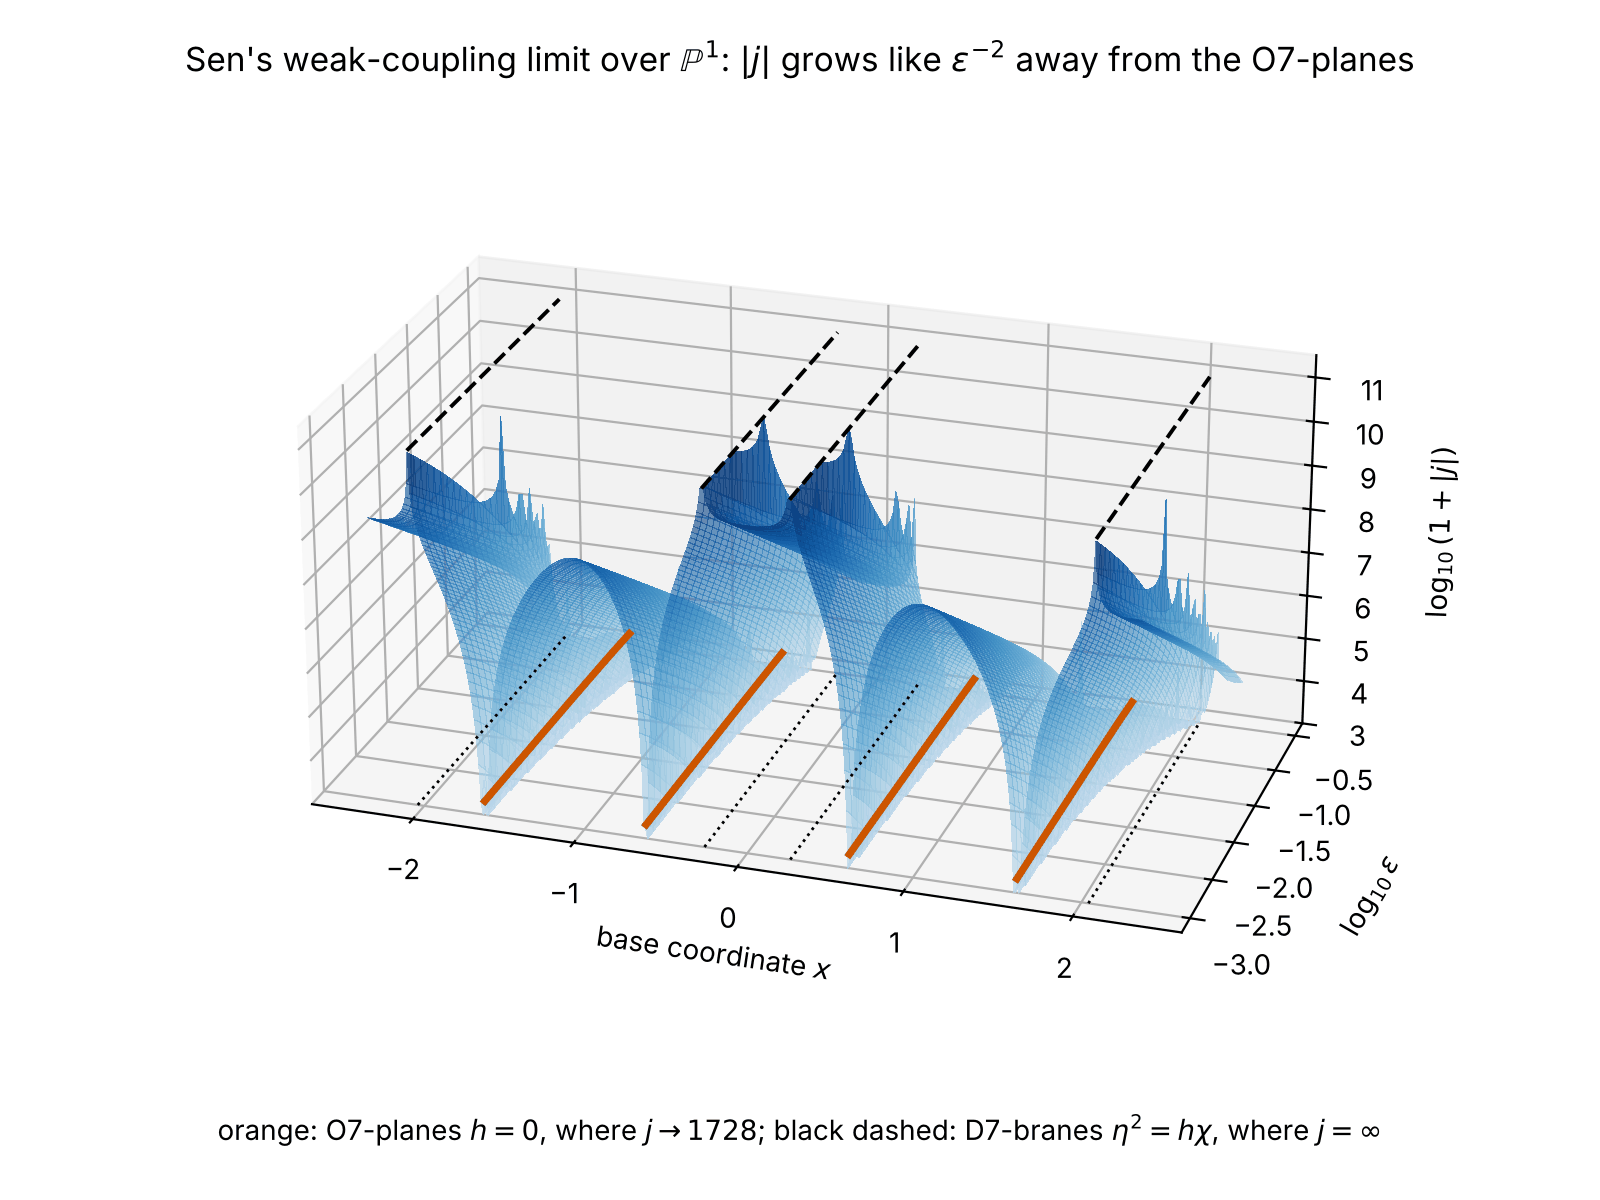
\includegraphics[width=0.94\linewidth,height=0.46\textheight,keepaspectratio]{figures/fig_weakcoupling.png}
\caption{Sen's K3 limit as a surface over the base coordinate $x$ of $\PP^1$ and the parameter $\eps$: the height is $\log_{10}(1+|j|)$ for $h=x^4-3x^2+1$, $\eta=x^8+2$, $\chi=3x^{12}+5$, sections of $L^2,L^4,L^6$ with $L=\mathcal O(2)$; values below $10^3$ are drawn on the floor. The coupling becomes weak, $|j|\sim\eps^{-2}$, everywhere except at the four O7-planes $h=0$ (orange lines), where $j\to1728$, and the four real D7-branes $\eta^2=h\chi$ (dashed), where $j$ has a pole for every $\eps$.}
\label{fig:weakcoupling}
\end{figure}

\begin{verdict}[claim 23]
Proved, in the form of Theorem~\ref{thm:normalform}: up to base change and rescaling, every weak coupling degeneration of F-theory on an elliptic Calabi--Yau is Sen's family, with the O7 divisor $h=0$ fixed by the limit point, and such a degeneration exists exactly when $h^0(-2K_B)>0$ (Corollary~\ref{cor:existence}). Sen calls the reduction formal and says that the auxiliary manifold can be singular; Proposition~\ref{prop:rigidcurves} and Corollary~\ref{cor:k3cover} identify when it is. Rigid curves of self-intersection $\le-5$ keep the coupling of order one and force a non-reduced branch divisor, and on surfaces the D7 singularity is a set of nodes. Beyond the geometry and the monodromies of Theorem~\ref{thm:senlimitk3}, \gap{the physical identification of the limit with a type IIB orientifold is not proved}; it remains a statement of string theory.
\end{verdict}
